% $Id: template.tex 11 2007-04-03 22:25:53Z jpeltier $


\documentclass{vgtc}                          % final (conference style)
%\documentclass[review]{vgtc}                 % review
%\documentclass[widereview]{vgtc}             % wide-spaced review
%\documentclass[preprint]{vgtc}               % preprint
%\documentclass[electronic]{vgtc}             % electronic version

%% Uncomment one of the lines above depending on where your paper is
%% in the conference process. ``review'' and ``widereview'' are for review
%% submission, ``preprint'' is for pre-publication, and the final version
%% doesn't use a specific qualifier. Further, ``electronic'' includes
%% hyperreferences for more convenient online viewing.

%% Please use one of the ``review'' options in combination with the
%% assigned online id (see below) ONLY if your paper uses a double blind
%% review process. Some conferences, like IEEE Vis and InfoVis, have NOT
%% in the past.

%% Figures should be in CMYK or Grey scale format, otherwise, colour 
%% shifting may occur during the printing process.

%% These few lines make a distinction between latex and pdflatex calls and they
%% bring in essential packages for graphics and font handling.
%% Note that due to the \DeclareGraphicsExtensions{} call it is no longer necessary
%% to provide the the path and extension of a graphics file:
%% 
\includegraphics{diamondrule} is completely sufficient.
%%
\ifpdf%                                % if we use pdflatex
  \pdfoutput=1\relax                   % create PDFs from pdfLaTeX
  \pdfcompresslevel=9                  % PDF Compression
  \pdfoptionpdfminorversion=7          % create PDF 1.7
  \ExecuteOptions{pdftex}
  \usepackage{graphicx}                % allow us to embed graphics files
  \DeclareGraphicsExtensions{.pdf,.png,.jpg,.jpeg} % for pdflatex we expect .pdf, .png, or .jpg files
\else%                                 % else we use pure latex
  \ExecuteOptions{dvips}
  \usepackage{graphicx}                % allow us to embed graphics files
  \DeclareGraphicsExtensions{.eps}     % for pure latex we expect eps files
\fi%

%% it is recomended to use ``\autoref{sec:bla}'' instead of ``Fig.~\ref{sec:bla}''
\graphicspath{size_and_scatterplots_files/figure-latex} % where to search for the images

\usepackage{microtype}                 % use micro-typography (slightly more compact, better to read)
\PassOptionsToPackage{warn}{textcomp}  % to address font issues with \textrightarrow
\usepackage{textcomp}                  % use better special symbols
\usepackage{mathptmx}                  % use matching math font
\usepackage{times}                     % we use Times as the main font
\renewcommand*\ttdefault{txtt}         % a nicer typewriter font
\usepackage{cite}                      % needed to automatically sort the references
\usepackage{tabu}                      % only used for the table example
\usepackage{booktabs}                  % only used for the table example
%% We encourage the use of mathptmx for consistent usage of times font
%% throughout the proceedings. However, if you encounter conflicts
%% with other math-related packages, you may want to disable it.


%% If you are submitting a paper to a conference for review with a double
%% blind reviewing process, please replace the value ``0'' below with your
%% OnlineID. Otherwise, you may safely leave it at ``0''.
\onlineid{0}

%% declare the category of your paper, only shown in review mode
\vgtccategory{Research}

%% allow for this line if you want the electronic option to work properly
\vgtcinsertpkg

%% In preprint mode you may define your own headline. If not, the default IEEE copyright message will appear in preprint mode.
%\preprinttext{To appear in an IEEE VGTC sponsored conference.}

%% This adds a link to the version of the paper on IEEEXplore
%% Uncomment this line when you produce a preprint version of the article 
%% after the article receives a DOI for the paper from IEEE
%\ieeedoi{xx.xxxx/TVCG.201x.xxxxxxx}


%% Paper title.

\title{Point Size and Correlation Perception in Scatterplots}

%% This is how authors are specified in the conference style

%% Author and Affiliation (single author).
%%\author{Roy G. Biv\thanks{e-mail: roy.g.biv@aol.com}}
%%\affiliation{\scriptsize Allied Widgets Research}

%% Author and Affiliation (multiple authors with single affiliations).
%%\author{Roy G. Biv\thanks{e-mail: roy.g.biv@aol.com} %
%%\and Ed Grimley\thanks{e-mail:ed.grimley@aol.com} %
%%\and Martha Stewart\thanks{e-mail:martha.stewart@marthastewart.com}}
%%\affiliation{\scriptsize Martha Stewart Enterprises \\ Microsoft Research}

%% Author and Affiliation (multiple authors with multiple affiliations)
\author{Gabriel Strain\thanks{\href{mailto:Gabriel.Strain@manchester.ac.uk}{\nolinkurl{Gabriel.Strain@manchester.ac.uk}}} %
\and Andrew J. Stewart\thanks{\href{mailto:Andrew.J.Stewart@manchester.ac.uk}{\nolinkurl{Andrew.J.Stewart@manchester.ac.uk}}} %
\and Paul Warren\thanks{\href{mailto:Paul.Warren@manchester.ac.uk}{\nolinkurl{Paul.Warren@manchester.ac.uk}}} %
\and Caroline Jay\thanks{\href{mailto:Caroline.Jay@manchester.ac.uk}{\nolinkurl{Caroline.Jay@manchester.ac.uk}}}} %
 \affiliation{\scriptsize The University of Manchester}


%% Abstract section.
\abstract{Place abstract here.}

%% ACM Computing Classification System (CCS). 
%% See <http://www.acm.org/about/class> for details.
%% We recommend the 2012 system <http://www.acm.org/about/class/class/2012>
%% For the 2012 system use the ``\CCScatTwelve'' which command takes four arguments.
%% The 1998 system <http://www.acm.org/about/class/class/2012> is still possible
%% For the 1998 system use the ``\CCScat'' which command takes four arguments.
%% In both cases the last two arguments (1998) or last three (2012) can be empty.

\CCScatlist{
  \CCScatTwelve{Human-centered computing}{Visu\-al\-iza\-tion}{Empirical studies in visualization};
  \CCScatTwelve{Human-centered computing}{Human computer interaction (HCI)}{Empirical studies in HCI}
}

%\CCScatlist{
  %\CCScat{H.5.2}{User Interfaces}{User Interfaces}{Graphical user interfaces (GUI)}{};
  %\CCScat{H.5.m}{Information Interfaces and Presentation}{Miscellaneous}{}{}
%}

%% Copyright space is enabled by default as required by guidelines.
%% It is disabled by the 'review' option or via the following command:
% \nocopyrightspace

%%%%%%%%%%%%%%%%%%%%%%%%%%%%%%%%%%%%%%%%%%%%%%%%%%%%%%%%%%%%%%%%
%%%%%%%%%%%%%%%%%%%%%% START OF THE PAPER %%%%%%%%%%%%%%%%%%%%%%
%%%%%%%%%%%%%%%%%%%%%%%%%%%%%%%%%%%%%%%%%%%%%%%%%%%%%%%%%%%%%%%%%

\begin{document}

%% The ``\maketitle'' command must be the first command after the
%% ``\begin{document}'' command. It prepares and prints the title block.

%% the only exception to this rule is the \firstsection command
\firstsection{Place intro here. Don't forget to put hypotheses}

\maketitle

\hypertarget{related-work}{%
\section{Related Work}\label{related-work}}

\hypertarget{correlation-perception}{%
\subsection{Correlation Perception}\label{correlation-perception}}

see Strain et al for a brief review of the history of correlation perception
testing with scatterplots

\hypertarget{point-size}{%
\subsection{Point Size}\label{point-size}}

Hong et al paper will be useful here

\hypertarget{dot-pitch-and-crowdsourced-experiments}{%
\subsection{Dot Pitch and Crowdsourced Experiments}\label{dot-pitch-and-crowdsourced-experiments}}

\hypertarget{methodology}{%
\section{Methodology}\label{methodology}}

\hypertarget{open-research-statement}{%
\subsection{Open Research Statement}\label{open-research-statement}}

The experiment was conducted according to the principles of open and reproducible research.
All data and analysis code are available at \url{https://github.com/gjpstrain/size_contrast_and_scatterplots}.
This repository contains instructions for building a docker image to fully
reproduce the computational environment used, allowing for full replications
of stimulus generation, analyses, and the paper itself. The experiment was
pre-registered with the OSF (\url{https://osf.io/k4gd8}).

\hypertarget{participants}{%
\subsection{Participants}\label{participants}}

150 participants were recruited using the Prolific.co platform. Normal to
corrected-to-normal vision and English fluency were required for participation. As in
\cite{strain_2023}, and in accordance with previously published guidelines \cite{peer_2021},
participants were required to have completed at least 100 studies on Prolific, and were
required to have a Prolific score of at least 100, indicating acceptance on at least
100/101 previously completed studies. Participants who took part in any of our
previous studies were prevented from participating.

\hypertarget{stimuli}{%
\subsection{Stimuli}\label{stimuli}}

The data used to generated the scatterplots in the current study was identical to that
in \cite{strain_2023}. They were generated based on 45 uniformly distributed \emph{r} values
between 0.2 and 0.99. Scatterplot points were generated based on bivariate normal
distributions with standard deviations of 1 in each direction. Each scatterplot
had a 1:1 aspect ratio, was generated as a 1200 x 1200 pixel .png image, and was
scaled up or down according to the participant's monitor. See section \ref{dot-pitch-and-crowdsourced-experiments}
for a more detailed discussion of precise point sizes and dot pitch in crowd-sourced
experiments.

As in our previous study \cite{strain_2023}, we used equation 1 to map residuals
to point sizes. We used a scaling factor of 4 and a constant of 0.2 to achieve a
minimum point size of 12/13 pixels, which is consistent with the point size on
a 1920 x 1080 monitor for both experiments in \cite{strain_2023}. Again, see section \ref{dot-pitch-and-crowdsourced-experiments}
for a discussion of dot pitch. Scripts detailing scatterplot and mask generation
can be found in the item preparation folder in the repository linked below.

\begin{equation}
  point-size = 1 - b^R
\end{equation}

\hypertarget{dot-pitch-and-crowdsourced-experiments-1}{%
\subsection{Dot Pitch and Crowdsourced Experiments}\label{dot-pitch-and-crowdsourced-experiments-1}}

In our previous study \cite{strain_2023}, we had no way of obtaining dot pitch
or participant to monitor distance due to the online, crowdsourced nature of the
experiments. Since then we have adopted a method for obtaining the height of a
participant's monitor in inches \cite{screenscale}. Combining this with the
monitor resolution fetched from Psychopy and assuming a widescreen 16:9 aspect ratio
allows us to infer dot pitch and therefore the physical size of the points in our
experiment. Mean dot pitch was 0.33 (\(SD = 0.06\)).
See section \ref{results} for analyses including dot pitch as a predictor.

\hypertarget{visual-threshold-testing}{%
\subsection{Visual Threshold Testing}\label{visual-threshold-testing}}

It is key that our manipulation does not functionally removing data from the scatterplot,
thus, in order to test that all our points were visible across a range of viewing
contexts and on a range of apparatus, we included visual threshold testing prior
to the experimental items in the study. Participants were shown six scatterplots
with a number of points, and were asked to enter in a textbox how many points
were being displayed. The points were the same size as the smallest points used
in the experimental materials. 5\% of
participants were correct on 5 out of 6 visual
threshold questions, while 95\% were correct
on 6 out of 6.

\hypertarget{design}{%
\subsection{Design}\label{design}}

The experiment used a fully repeated measures, within-participants design, with each
participant seeing and responding to each of the 180 scatterplots in a randomised order.
There were four scatterplots for each of the 45 \emph{r} values corresponding to the
four levels of the size condition, examples of which can be see in figure \ref{fig:examples}.
Everything needed to run the experiment, including code, materials, instructions, and scripts, is
hosted at \url{https://gitlab.pavlovia.org/Strain/exp_size_only}.

\begin{figure}
\centering
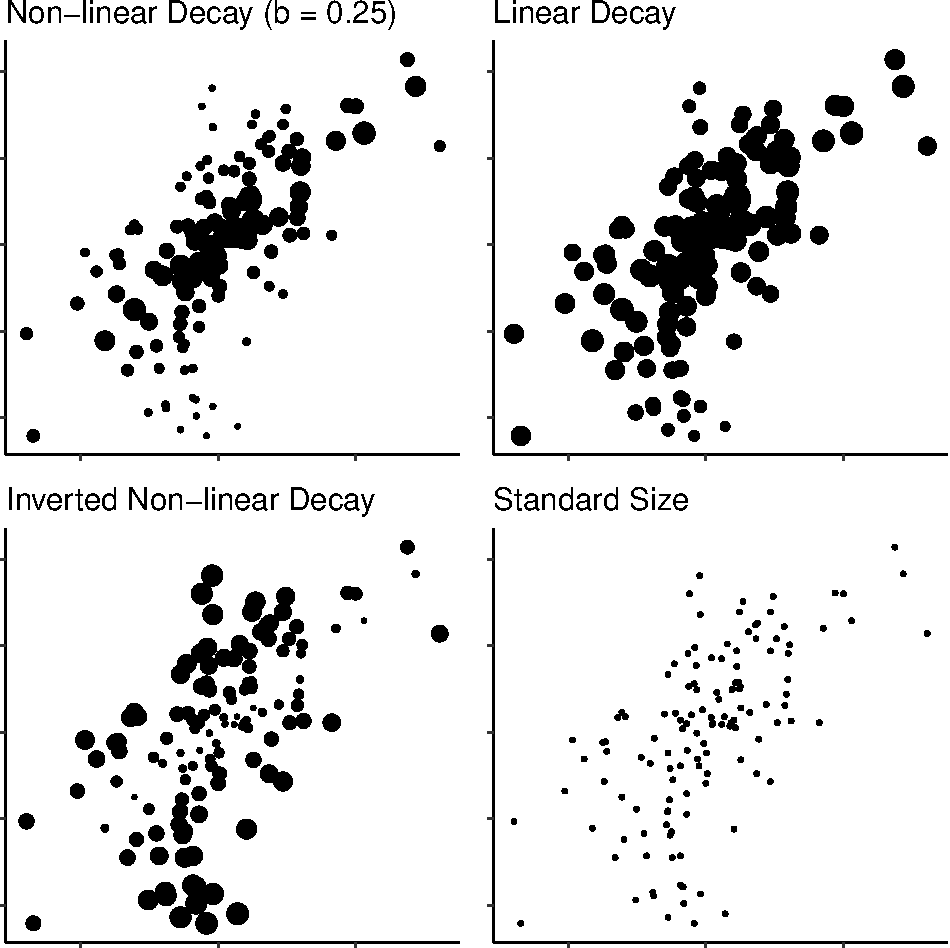
\includegraphics{size_and_scatterplots_files/figure-latex/examples-1.pdf}
\caption{\label{fig:examples}Four levels of the point size condition, demonstrated with an \textit{r} value of 0.6}
\end{figure}

\hypertarget{results}{%
\section{Results}\label{results}}

include short discussion of modelling paradigm and justification for it

\hypertarget{discussion}{%
\section{Discussion}\label{discussion}}

\begin{figure*}

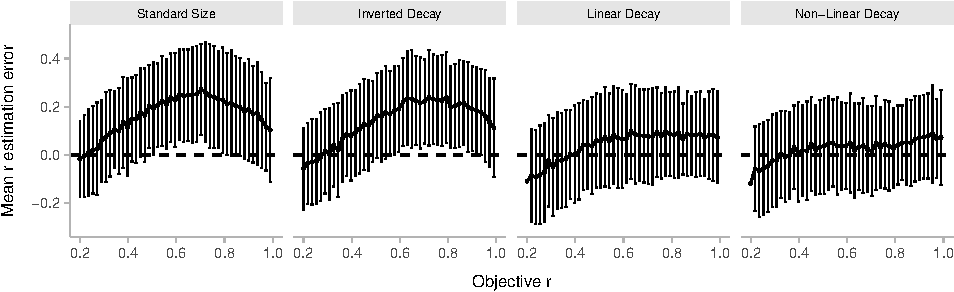
\includegraphics{size_and_scatterplots_files/figure-latex/changes-with-r-size-1} \hfill{}

\caption{hello}\label{fig:changes-with-r-size}
\end{figure*}

\begin{figure*}

{\centering 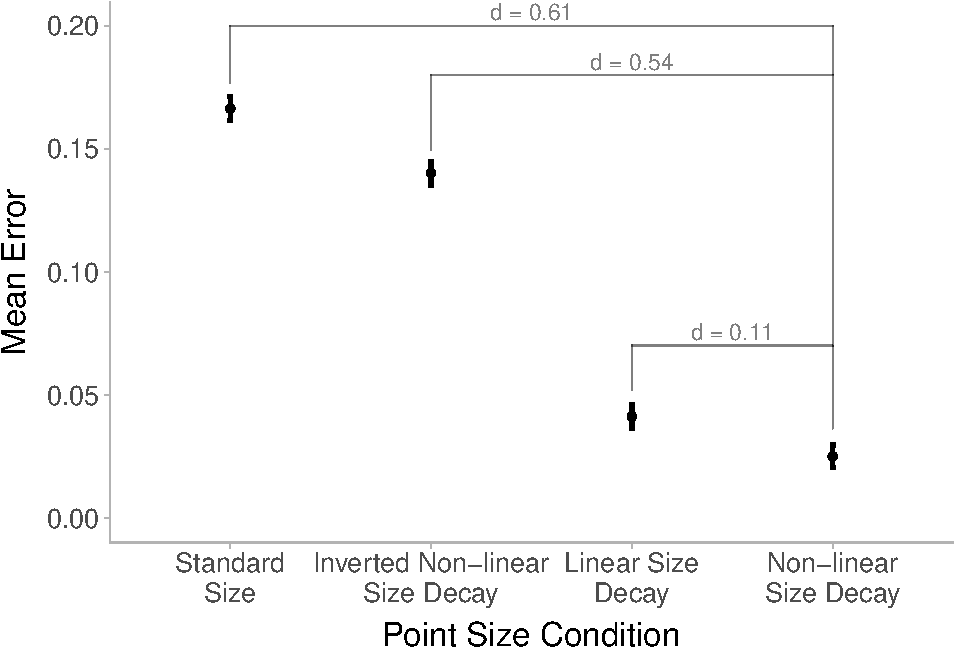
\includegraphics{size_and_scatterplots_files/figure-latex/dot-plot-1} 

}

\caption{hello}\label{fig:dot-plot}
\end{figure*}

%% if specified like this the section will be committed in review mode
\acknowledgments{lah di dah}

%\bibliographystyle{abbrv}
\bibliographystyle{abbrv-doi}
%\bibliographystyle{abbrv-doi-narrow}
%\bibliographystyle{abbrv-doi-hyperref}
%\bibliographystyle{abbrv-doi-hyperref-narrow}

\bibliography{size\_contrast\_scatterplots.bib}
\end{document}
